\documentclass[11pt]{article}
% ===========================================================================
%  Shared preamble for all MPM2D worksheets — input right after \documentclass.
%  (Files beginning with "_" are skipped by mpm2d-worksheet-publish.mjs.)
% ===========================================================================
\usepackage[letterpaper,top=2.2cm,bottom=1.9cm,left=1.6cm,right=1.6cm,headheight=28pt,footskip=24pt]{geometry}
\usepackage{amsmath,amssymb}
\usepackage[T1]{fontenc}
\usepackage[utf8]{inputenc}
\usepackage{lmodern}
\usepackage{xcolor}
\usepackage[most]{tcolorbox}
\usepackage{enumitem}
\usepackage{multicol}
\usepackage{fancyhdr}
\usepackage{tikz}
\usetikzlibrary{calc}
\usepackage{pgfplots}
\pgfplotsset{compat=1.18}

\definecolor{exblue}{HTML}{4A90E2}
\definecolor{exbg}{HTML}{E6F3FF}
\definecolor{qorange}{HTML}{E69138}
\definecolor{qbg}{HTML}{FFF7CC}
\definecolor{keygray}{HTML}{475569}
\definecolor{keybg}{HTML}{F1F5F9}
\definecolor{iagreen}{HTML}{14653B}
\definecolor{titleblue}{HTML}{1D4ED8}
% Rotating palette so each worked example gets its own colour.
\definecolor{ex0}{HTML}{2563A0}\definecolor{ex1}{HTML}{3B7D3B}\definecolor{ex2}{HTML}{8A5A00}
\definecolor{ex3}{HTML}{A3327A}\definecolor{ex4}{HTML}{6D28A3}\definecolor{ex5}{HTML}{B08900}
\definecolor{ex6}{HTML}{0E7490}\definecolor{ex7}{HTML}{9A3412}\definecolor{ex8}{HTML}{15803D}

\pagestyle{fancy}
\fancyhf{}
\fancyhead[L]{\footnotesize NAME: \underline{\hspace{3.4cm}}}
\fancyhead[C]{\textbf{Integration Academy}\\[-2pt]{\scriptsize Math Simplified \textperiodcentered{} Success Amplified}}
\fancyhead[R]{\footnotesize MPM2D}
\fancyfoot[L]{\scriptsize dr.merie@IntegrationAcademy.ca}
\fancyfoot[C]{\scriptsize\thepage}
\fancyfoot[R]{\scriptsize IntegrationAcademy.ca}
\renewcommand{\headrulewidth}{1.2pt}
\renewcommand{\footrulewidth}{0.4pt}
\setlength{\parindent}{0pt}
\setlength{\parskip}{4pt}

% Examples are NOT breakable, so each example + its solution stays on one page.
\newtcolorbox{example}[2]{colframe=#1,colback=#1!7,coltitle=white,colbacktitle=#1,fonttitle=\bfseries,title={#2},arc=3pt,boxrule=1pt}
\newtcolorbox{qbox}[1]{colframe=qorange,colback=qbg,coltitle=white,colbacktitle=qorange,fonttitle=\bfseries,title={#1},arc=3pt,breakable,boxrule=1pt}
\newtcolorbox{keybox}{colframe=keygray,colback=keybg,coltitle=white,colbacktitle=keygray,fonttitle=\bfseries,title={$\checkmark$\ Answer Key},arc=3pt,breakable,boxrule=1pt}
\newtcolorbox{recapbox}{colframe=keygray,colback=keybg,coltitle=white,colbacktitle=keygray,fonttitle=\bfseries,title={Question Recap},arc=3pt,breakable,boxrule=1pt}
\newtcolorbox{ideabox}{colframe=titleblue,colback=titleblue!6,coltitle=white,colbacktitle=titleblue,fonttitle=\bfseries,title={The Big Ideas},arc=3pt,breakable,boxrule=1.2pt}
\newtcolorbox{learnbox}{colframe=iagreen,colback=iagreen!5,coltitle=white,colbacktitle=iagreen,fonttitle=\bfseries,title={Concept Essentials},arc=3pt,breakable,boxrule=1.2pt}
\newcommand{\lh}[1]{\par\smallskip{\bfseries\color{iagreen}#1}\par\nobreak\smallskip}

\newcommand{\soln}{\par\smallskip\textit{\textbf{Solution.}}\ }
\newcommand{\workspace}[1]{\par\vspace{3pt}\fcolorbox{black!30}{white}{\begin{minipage}[t][#1][t]{\dimexpr\linewidth-2\fboxsep\relax}\ \end{minipage}}\par}
\newcommand{\sech}[1]{\par\vspace{8pt}{\Large\bfseries\color{iagreen}#1}\par\nobreak\vspace{2pt}{\color{black!20}\hrule height1pt}\vspace{6pt}}

% A compact coordinate plot sized for an example box: \eplot{xmin}{xmax}{ymin}{ymax}{body}
\newcommand{\eplot}[5]{\begin{center}\begin{tikzpicture}
\begin{axis}[width=6.8cm,height=4.4cm,axis lines=middle,xlabel={\tiny$x$},ylabel={\tiny$y$},
grid=both,grid style={gray!16},xmin=#1,xmax=#2,ymin=#3,ymax=#4,
xtick distance=2,ytick distance=2,tick label style={font=\tiny},axis line style={-},samples=120]
#5
\end{axis}\end{tikzpicture}\end{center}}

% A sine-curve plot (degrees on x, 0..360): \splot{ymin}{ymax}{body}
\newcommand{\splot}[3]{\begin{center}\begin{tikzpicture}
\begin{axis}[width=8.6cm,height=4.6cm,axis lines=middle,xlabel={\tiny$x\,(^\circ)$},ylabel={\tiny$y$},
grid=both,grid style={gray!16},xmin=0,xmax=360,ymin=#1,ymax=#2,
xtick distance=90,ytick distance=1,tick label style={font=\tiny},axis line style={-},samples=180]
#3
\end{axis}\end{tikzpicture}\end{center}}

% A small coordinate plot: \plot{xmin}{xmax}{ymin}{ymax}{body}
\newcommand{\plot}[5]{\begin{center}\begin{tikzpicture}
\begin{axis}[width=8.4cm,height=6cm,axis lines=middle,xlabel={\scriptsize$x$},ylabel={\scriptsize$y$},
grid=both,grid style={gray!16},xmin=#1,xmax=#2,ymin=#3,ymax=#4,
xtick distance=2,ytick distance=2,tick label style={font=\tiny},axis line style={-}]
#5
\end{axis}\end{tikzpicture}\end{center}}

% Right triangle (angle theta at bottom-left, right angle at bottom-right):
%   \rtri{drawBase}{drawHeight}{oppLabel}{adjLabel}{hypLabel}
\newcommand{\rtri}[5]{\begin{center}\begin{tikzpicture}[scale=0.85]
\coordinate (A) at (0,0);\coordinate (B) at (#1,0);\coordinate (C) at (#1,#2);
\draw[thick,exblue] (A)--(B)--(C)--cycle;
\draw[black] ($(B)+(-0.32,0)$)--($(B)+(-0.32,0.32)$)--($(B)+(0,0.32)$);
\node[below] at ($(A)!0.5!(B)$){#4};
\node[right] at ($(B)!0.5!(C)$){#3};
\node[above left] at ($(A)!0.5!(C)$){#5};
\node at (0.7,0.22){$\theta$};
\end{tikzpicture}\end{center}}

% General (oblique) triangle with vertex labels and opposite-side labels:
%   \gtri{Alabel}{Blabel}{Clabel}{aSide}{bSide}{cSide}
\newcommand{\gtri}[6]{\begin{center}\begin{tikzpicture}[scale=0.85]
\coordinate (A) at (0,0);\coordinate (B) at (5,0);\coordinate (C) at (1.6,3);
\draw[thick,exblue] (A)--(B)--(C)--cycle;
\node[below left] at (A){#1};\node[below right] at (B){#2};\node[above] at (C){#3};
\node[below] at ($(A)!0.5!(B)$){#6};
\node[right] at ($(B)!0.5!(C)$){#4};
\node[left] at ($(A)!0.5!(C)$){#5};
\end{tikzpicture}\end{center}}

\fancyhead[R]{\footnotesize MCR3U \textperiodcentered{} 2.1}
\begin{document}

\begin{center}
{\LARGE\bfseries\color{titleblue}Worksheet 2.1 --- Adding \& Multiplying Polynomials}\\[2pt]
{\small Grade 11 Functions, University (MCR3U) \textperiodcentered{} Unit 2: Equivalent Algebraic Expressions}
\end{center}

\begin{ideabox}
Two expressions are \textbf{equivalent} when they have the same value for every $x$ --- so they draw the \emph{same graph}. Rewriting by collecting like terms and expanding products is how we turn one form into another without changing its value. Every rewrite below is tested: by substituting numbers, and by comparing graphs.
\begin{itemize}[leftmargin=*,itemsep=2pt]
  \item \textbf{Like terms} (same variable part) combine; a minus sign before a bracket flips \emph{every} sign inside.
  \item \textbf{Distribute:} every term of one factor meets every term of the other. The \textbf{area model} keeps score; FOIL is its shortcut for two binomials.
  \item \textbf{Special products:} $(a\pm b)^2=a^2\pm2ab+b^2$ and $(a+b)(a-b)=a^2-b^2$.
  \item \textbf{Degrees:} the degree of a product is the \emph{sum} of the degrees; the degree of a sum is at most the larger one.
  \item \textbf{Test it:} one mismatch proves two expressions are \emph{not} equivalent; a match at every tested value (or a single overlapping graph) supports --- and algebra proves --- equivalence.
\end{itemize}
\end{ideabox}

\begin{learnbox}
\lh{Equivalent means the same graph}Two expressions are equivalent if they give the same output for every $x$. Rewriting (collecting like terms, expanding) must never change the value: \textbf{test} a rewrite by substituting numbers --- one mismatch proves it wrong.
\lh{Expanding}Every term in one factor multiplies every term in the other. An \textbf{area model} lays the partial products in a grid; \textbf{like terms} (same colour) are then collected. Degrees \emph{add} when you multiply.
\lh{Special products}$(a+b)^2=a^2+2ab+b^2$, $(a-b)^2=a^2-2ab+b^2$, $(a+b)(a-b)=a^2-b^2$. They are shortcuts you will use \emph{backwards} when factoring in 2.2.
\end{learnbox}

\sech{Worked Examples}

\begin{example}{ex0}{Example 1 --- Adding polynomials}
Simplify $(4x^3-2x+7)+(x^3+5x^2-3x-9)$.\soln Group like terms by degree: $(4x^3+x^3)+5x^2+(-2x-3x)+(7-9)$. \\ $=5x^3 + 5x^2 - 5x - 2$.
\end{example}

\begin{example}{ex1}{Example 2 --- Distribute, then collect}
Simplify $3(2x-1)-4(x-5)+2x(x+3)$.\soln Distribute: $6x-3-4x+20+2x^2+6x$. \\ Note the $-4$ multiplies \emph{both} terms: $-4\cdot(-5)=+20$. \\ Collect: $2x^2 + 8x + 17$.
\end{example}

\begin{example}{ex2}{Example 3 --- Area model}
Expand $(2x+1)(x+6)$.\soln The boxes are $2x\cdot x=2x^2$, $2x\cdot6=12x$, $1\cdot x=x$, $1\cdot6=6$. \\ The two $x$-boxes are like terms: $12x+x=13x$. \\ $=2x^2 + 13x + 6$.
\end{example}

\begin{example}{ex3}{Example 4 --- FOIL with a negative}
Expand $(4x-5)(2x+3)$.\soln First $8x^2$; Outer $12x$; Inner $-10x$; Last $-15$. \\ Middle: $12x-10x=2x$. \\ $=8x^2 + 2x - 15$.
\end{example}

\begin{example}{ex4}{Example 5 --- Special products}
Expand (a) $(6x-1)^2$ and (b) $(2x+9)(2x-9)$.\soln (a) $(6x)^2-2(6x)(1)+1^2=36x^2 - 12x + 1$. \\ (b) The middle terms $\pm18x$ cancel: $(2x)^2-9^2=4x^2 - 81$.
\end{example}

\begin{example}{ex5}{Example 6 --- Trinomial times binomial}
Expand $(2x^2+x-4)(x-3)$.\soln Six partial products: $2x^3-6x^2+x^2-3x-4x+12$. \\ Collect: $2x^3 - 5x^2 - 7x + 12$. \\ Check the degree ($2+1=3$) and the constant term ($-4\cdot-3=12$).
\end{example}

\begin{example}{ex6}{Example 7 --- A power of a binomial}
Expand $(x+1)^4$.\soln The coefficients are Pascal's row $1,4,6,4,1$ and every power of $1$ is $1$. \\ $=x^4 + 4x^3 + 6x^2 + 4x + 1$. \\ Check at $x=1$: $2^4=16$ and $1+4+6+4+1=16$.
\end{example}

\begin{example}{ex7}{Example 8 --- Application: a picture frame}
A photo is $30$ cm by $20$ cm. A frame of width $x$ goes all the way around it. Write the area of the frame alone.\soln Outer rectangle: $(30+2x)(20+2x)$. Subtract the photo, $600$. \\ $(30+2x)(20+2x)-600=600+100x+4x^2-600=4x^2 + 100x$. \\ For a $2$ cm frame: $4(4)+100(2)=216$ cm$^2$.
\end{example}

\begin{example}{ex8}{Example 9 --- Are they equivalent?}
Test whether $(x+2)^2-(x-2)^2$ and $8x$ are equivalent.
\begin{center}\renewcommand{\arraystretch}{1.35}\setlength{\tabcolsep}{3pt}\begin{tabular}{l|ccccc}
$x$ & $-2$ & $-1$ & $0$ & $1$ & $2$ \\ \hline
$(x+2)^2-(x-2)^2$ & \makebox[1.35cm]{\strut $-16$} & \makebox[1.35cm]{\strut $-8$} & \makebox[1.35cm]{\strut $0$} & \makebox[1.35cm]{\strut $8$} & \makebox[1.35cm]{\strut $16$} \\
$8x$ & \makebox[1.35cm]{\strut $-16$} & \makebox[1.35cm]{\strut $-8$} & \makebox[1.35cm]{\strut $0$} & \makebox[1.35cm]{\strut $8$} & \makebox[1.35cm]{\strut $16$} \\
\hline same? & \makebox[1.35cm]{\strut $\checkmark$} & \makebox[1.35cm]{\strut $\checkmark$} & \makebox[1.35cm]{\strut $\checkmark$} & \makebox[1.35cm]{\strut $\checkmark$} & \makebox[1.35cm]{\strut $\checkmark$} \\
\end{tabular}\end{center}
\soln The values match at all five points. To \emph{prove} it, expand: $(x^2+4x+4)-(x^2-4x+4)=8x$ --- the $x^2$ and constants cancel.\begin{center}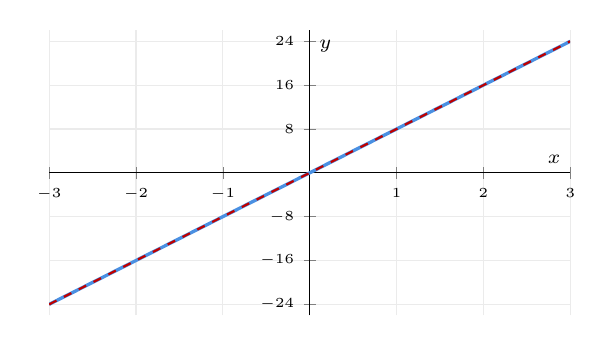
\begin{tikzpicture}\begin{axis}[width=8.2cm,height=5.2cm,axis lines=middle,xlabel={\scriptsize$x$},ylabel={\scriptsize$y$},grid=both,grid style={gray!16},xmin=-3,xmax=3,ymin=-26,ymax=26,xtick distance=1,ytick distance=8,tick label style={font=\tiny},axis line style={-}]
\addplot[exblue,very thick,domain=-3:3,samples=120,restrict y to domain=-27:27]{(x+2)^2-(x-2)^2};
\addplot[red!75!black,dashed,thick,domain=-3:3,samples=120,restrict y to domain=-27:27]{8*x};
\end{axis}\end{tikzpicture}\\[-2pt]{\scriptsize Both expressions draw the same line, so the dashed graph lies exactly on the solid one.}\end{center}
\end{example}

\clearpage
\sech{Your Turn --- Show Your Work}
For each question, show all steps clearly in the space provided.

\begin{qbox}{Question 1}
Simplify $(7x^2-3x+4)-(3x^2-x+12)$. Then test your answer at $x=2$.\workspace{2.6cm}
\end{qbox}

\begin{qbox}{Question 2}
Expand $-3x(5x^2-2x-1)$.\workspace{2.2cm}
\end{qbox}

\begin{qbox}{Question 3}
Expand and simplify $(5x-3)(2x+7)$ using an area model.\workspace{3.6cm}
\end{qbox}

\begin{qbox}{Question 4}
Expand (a) $(7x+4)^2$ \quad (b) $(5x+6)(5x-6)$. Explain why (b) has no $x$-term.\workspace{3.6cm}
\end{qbox}

\begin{qbox}{Question 5}
Expand $(3x^2-2x-6)(x-4)$.\workspace{3.8cm}
\end{qbox}

\begin{qbox}{Question 6}
Expand $(x-4)^3$ using $(x-4)^3=(x-4)(x-4)^2$. Check your answer at $x=5$.\workspace{3.8cm}
\end{qbox}

\begin{qbox}{Question 7}
Simplify $(x+9)^2-(x-3)^2$. Which special-product pattern gives a quicker route?\workspace{3.2cm}
\end{qbox}

\begin{qbox}{Question 8}
Expand and simplify $(x+2)(x-3)(x+4)$.\workspace{4.2cm}
\end{qbox}

\begin{qbox}{Question 9}
Expand $(2x-3)(x^2-2x-8)$ and state the degree and the constant term \emph{before} you multiply. Do they match your result?\workspace{4cm}
\end{qbox}

\begin{qbox}{Question 10}
Complete the table to decide whether $(x-3)^2$ is equivalent to (a) $x^2-9$ or (b) $x^2-6x+9$. Then expand to confirm.
\begin{center}\renewcommand{\arraystretch}{1.35}\setlength{\tabcolsep}{3pt}\begin{tabular}{l|ccccc}
$x$ & $-1$ & $0$ & $1$ & $2$ & $3$ \\ \hline
$(x-3)^2$ & \makebox[1.35cm]{\strut } & \makebox[1.35cm]{\strut } & \makebox[1.35cm]{\strut } & \makebox[1.35cm]{\strut } & \makebox[1.35cm]{\strut } \\
$x^2-9$ & \makebox[1.35cm]{\strut } & \makebox[1.35cm]{\strut } & \makebox[1.35cm]{\strut } & \makebox[1.35cm]{\strut } & \makebox[1.35cm]{\strut } \\
$x^2-6x+9$ & \makebox[1.35cm]{\strut } & \makebox[1.35cm]{\strut } & \makebox[1.35cm]{\strut } & \makebox[1.35cm]{\strut } & \makebox[1.35cm]{\strut } \\
\hline same? & \makebox[1.35cm]{\strut } & \makebox[1.35cm]{\strut } & \makebox[1.35cm]{\strut } & \makebox[1.35cm]{\strut } & \makebox[1.35cm]{\strut } \\
\end{tabular}\end{center}\workspace{2.2cm}
\end{qbox}

\begin{qbox}{Question 11}
A student writes $(2x+1)^2-(x-3)(x+3)=3x^2+4x-8$. Find the error and give the correct simplified answer.\workspace{3.4cm}
\end{qbox}

\begin{qbox}{Question 12}
A $24$ cm by $18$ cm sheet has squares of side $x$ cut from each corner and the sides folded to make an open box. Write the volume as an expanded polynomial and find $V$ when $x=3$.\workspace{4cm}
\end{qbox}

\begin{qbox}{Question 13}
Explain in a sentence or two why the degree of $(x^3+x)+(-x^3+2x^2)$ is smaller than the degree of either bracket. Give your own example of a sum of two cubics that is a quadratic.\workspace{3cm}
\end{qbox}

\begin{qbox}{Question 14 --- Challenge}
Show that $n^2+(n+1)^2$ is always odd, for any integer $n$. Then show that $(n+1)^2-n^2$ equals the sum of the two numbers $n$ and $n+1$.\workspace{4.2cm}
\end{qbox}

\clearpage
\sech{Question Recap \& Answer Key}

\begin{recapbox}
\begin{multicols}{2}
\small
\begin{enumerate}[leftmargin=*,itemsep=3pt]
  \item Simplify $(7x^2-3x+4)-(3x^2-x+12)$. Then test your answer at $x=2$.
  \item Expand $-3x(5x^2-2x-1)$.
  \item Expand and simplify $(5x-3)(2x+7)$ using an area model.
  \item Expand (a) $(7x+4)^2$ \quad (b) $(5x+6)(5x-6)$. Explain why (b) has no $x$-term.
  \item Expand $(3x^2-2x-6)(x-4)$.
  \item Expand $(x-4)^3$ using $(x-4)^3=(x-4)(x-4)^2$. Check your answer at $x=5$.
  \item Simplify $(x+9)^2-(x-3)^2$. Which special-product pattern gives a quicker route?
  \item Expand and simplify $(x+2)(x-3)(x+4)$.
  \item Expand $(2x-3)(x^2-2x-8)$ and state the degree and the constant term \emph{before} you multiply. Do they match your result?
  \item Complete the table to decide whether $(x-3)^2$ is equivalent to (a) $x^2-9$ or (b) $x^2-6x+9$. Then expand to confirm.
\begin{center}\renewcommand{\arraystretch}{1.35}\setlength{\tabcolsep}{3pt}\begin{tabular}{l|ccccc}
$x$ & $-1$ & $0$ & $1$ & $2$ & $3$ \\ \hline
$(x-3)^2$ & \makebox[1.35cm]{\strut } & \makebox[1.35cm]{\strut } & \makebox[1.35cm]{\strut } & \makebox[1.35cm]{\strut } & \makebox[1.35cm]{\strut } \\
$x^2-9$ & \makebox[1.35cm]{\strut } & \makebox[1.35cm]{\strut } & \makebox[1.35cm]{\strut } & \makebox[1.35cm]{\strut } & \makebox[1.35cm]{\strut } \\
$x^2-6x+9$ & \makebox[1.35cm]{\strut } & \makebox[1.35cm]{\strut } & \makebox[1.35cm]{\strut } & \makebox[1.35cm]{\strut } & \makebox[1.35cm]{\strut } \\
\hline same? & \makebox[1.35cm]{\strut } & \makebox[1.35cm]{\strut } & \makebox[1.35cm]{\strut } & \makebox[1.35cm]{\strut } & \makebox[1.35cm]{\strut } \\
\end{tabular}\end{center}
  \item A student writes $(2x+1)^2-(x-3)(x+3)=3x^2+4x-8$. Find the error and give the correct simplified answer.
  \item A $24$ cm by $18$ cm sheet has squares of side $x$ cut from each corner and the sides folded to make an open box. Write the volume as an expanded polynomial and find $V$ when $x=3$.
  \item Explain in a sentence or two why the degree of $(x^3+x)+(-x^3+2x^2)$ is smaller than the degree of either bracket. Give your own example of a sum of two cubics that is a quadratic.
  \item Show that $n^2+(n+1)^2$ is always odd, for any integer $n$. Then show that $(n+1)^2-n^2$ equals the sum of the two numbers $n$ and $n+1$.
\end{enumerate}
\end{multicols}
\end{recapbox}

\begin{keybox}
\begin{multicols}{2}
\small
\begin{enumerate}[leftmargin=*,itemsep=3pt]
  \item $4x^2 - 2x - 8$. At $x=2$: original $(28-6+4)-(12-2+12)=26-22=4$; answer $16-4-8=4$.
  \item $-15x^3 + 6x^2 + 3x$.
  \item $10x^2 + 29x - 21$ (boxes $10x^2,\ 35x,\ -6x,\ -21$).
  \item (a) $49x^2 + 56x + 16$ \quad (b) $25x^2 - 36$. The two middle terms $\pm30x$ are opposites and cancel.
  \item $3x^3 - 14x^2 + 2x + 24$.
  \item $x^3 - 12x^2 + 48x - 64$. At $x=5$: $(1)^3=1$ and $125-300+240-64=1$.
  \item $24x + 72$. Difference of squares with $a=x+9,\ b=x-3$: $(a-b)(a+b)=12(2x+6)=24x+72$.
  \item $x^3 + 3x^2 - 10x - 24$.
  \item Degree $1+2=3$, constant term $(-3)(-8)=24$. Result $2x^3 - 7x^2 - 10x + 24$ \quad \checkmark.
  \item Row values: $(x-3)^2$: $16,9,4,1,0$; $x^2-9$: $-8,-9,-8,-5,0$; $x^2-6x+9$: $16,9,4,1,0$. So (b) is equivalent, (a) is not. Expanding $(x-3)(x-3)$ gives $x^2-6x+9$.
  \item $(2x+1)^2=4x^2+4x+1$ and $(x-3)(x+3)=x^2-9$, so the subtraction gives $4x^2+4x+1-x^2+9$. The student wrote $-8$ instead of $+10$ (forgot the minus flips $-9$ to $+9$). Correct: $3x^2 + 4x + 10$.
  \item $V=x(30-2x)(20-2x)=4x^3 - 84x^2 + 432x$. At $x=3$: $3\cdot18\cdot12=648$ cm$^3$; check $108-756+1296=648$.
  \item The $x^3$ terms cancel ($x^3-x^3$), leaving $2x^2+x$. A sum can have lower degree than its parts. Example: $(x^3+4x)+(-x^3+x^2)=x^2+4x$.
  \item $n^2+(n+1)^2=2n^2+2n+1=2(n^2+n)+1$, which is $2\times$ an integer plus $1$: odd. And $(n+1)^2-n^2=2n+1=n+(n+1)$.
\end{enumerate}
\end{multicols}
\end{keybox}

\end{document}
